The lunar farside provides a unique accessible environment in that the moon shields it from Earth and near-Earth RFI at all times. Therefore, {\em anything} detected is of scientific interest. Since there is no ionospheric blockage, low frequency observations that are impossible from Earth can also be made in an RFI-free environment. Although the lunar farside will remain an excellent low-RFI site for many years to come, {\em now} is the only time to take completely pristine measurements of the radio spectrum. This is an opportunity that will never again present itself, as seen in Fig.\ \ref{fig:missions}.  This section summarizes the primary science cases that drive the design of the array, which is summarized in the science traceability matrix in Appendix A.

\subsection{Technosignatures}
Humanity's quest to determine its place in the Universe and whether we are its only inhabitants has driven knowledge and imagination since we first looked to the sky.  Many large telescopes are in consideration in order to help determine if other biological processes are happening in nearby stars (called "biosignatures") and we now also have the capability to explore whether technological signals (``technosignatures'') exist over a large swath of our Galaxy.  The Breakthrough Listen program has transformed the field and has greatly expanded the search for such technosignatures (e.g. \citealt{Enriquez_2017, Price_2020, Gajjar_2021}).  The greatest impediment is the prevalence of RFI made by essentially every device that is electrically powered.

Although RFI is prevalent, excellent technosignature searches can be conducted from the earth, particularly from remote locations where terrestrial interference is low and in frequencies that, at that time, place and frequency, are free of interfering signals. See Figure \ref{fig:bubbles} where the circles represent the ground-based radio searches that have been done and the highlighted regions of two of the large program (purple and red shaded regions) technosignature searches in progress. In order to further guard against temporary interference one usually uses a cadence of a series of on-targets and off-targets, where the ``off'' can be the ``on'' for another target. The use of this in a multi-beam system as outlined in Figure \ref{fig:midband_beam_maps} is demostrated in \cite{Huang_2023}. Note that using a multi-beam system allows for the ``on'' and ``off'' to be simultaneous, making it even more efficient (i.e., \citealt{multibeam}). A significant amount of detection time is, however, highly desirable. Also, note that a remote site doesn't provide shielding from satellites and airplanes. Techniques do exist to subtract or decorrelate interference, however they are not perfect and it seems unlikely that a technosignature detection ``through'' RFI would be believed -- even if not immediately rejected in a pipeline, as would likely be the case.

\begin{figure}
    \centering
    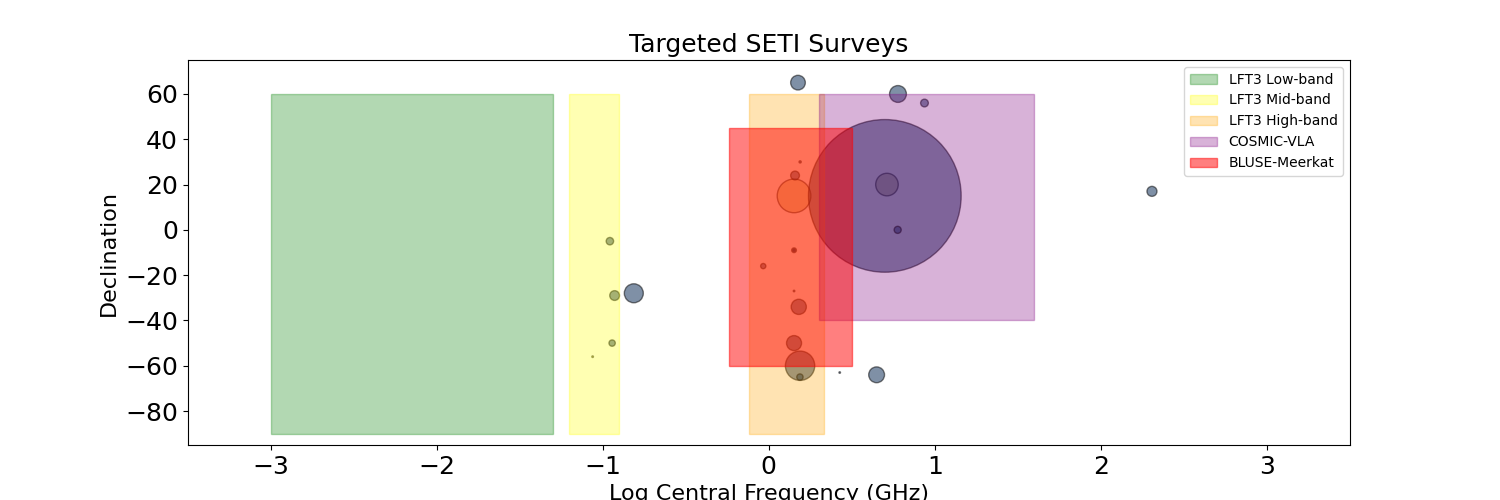
\includegraphics[width=0.85\linewidth]{SETI_Bubble_LFT3.png}
    \caption{A plot of the historical technosignature searches modified from \cite{Tremblay_2022}. The circles size is scaled to the total number of targetted sources within the survey. The colored rectangles show the regions in frequency and declination that LFT3 will cover as well as two large ground-based programs. As shown, LFT3 will survey regions that cover both new or rare regions (low and mid bands) as well as well studied regions (high-band).}
    \label{fig:bubbles}
\end{figure}

Of course, we don't have any information on any parameter of a technosignature, so one must search agnostically with the most sensitive receivers one can muster.  However, we do know that the most likely initial signal detected will have a high signal-to-noise in some parameter space. For now, at radio wavelengths, that parameter space is frequency space and narrow-band signals are the most likely to be detected.  Additionally, they are among the least likely signals to be confused with an astrophysical process. There is a case to be made, that the most likely initial detection will be a slow transient arising from some underlying cadence such as a civilization targeting many distant worlds with a beacon or some fortuitous alignment such as the conjunction of two extrasolar planets with our telescope beam.  As mentioned in the Introduction, the ``Wow!'' signal is an exemplar of what one such signal could look like.  As also mentioned, if observed from the earth even if that event occured where it wasn't obscured by RFI one would likely not have a high confidence of its origin due to the many other sources of potential short-term RFI. To reliably detect such a signal one must go to a place with no other potential sources.

In order to assess if a small telescope can meaningfully search for technosignatures it is instructive to look at detectability of various transmitter strengths for the stellar distribution around us. The Arecibo planetary radar has been the highest effective isotropic power radiator at a level of greater than 20 TW and is a key fiducial. Another is to assume that an advanced civilization could produce significantly greater radiated power, in this case we will use 1000 times the Arecibo planetary radar.  Figure \ref{fig:isaacsonetal} shows the signal-to-noise ratios if these transmitters were at the location of stars in various star catalogs.  As shown, even our current technology provides a detectable signal to this telescope.

\begin{figure}
    \centering
    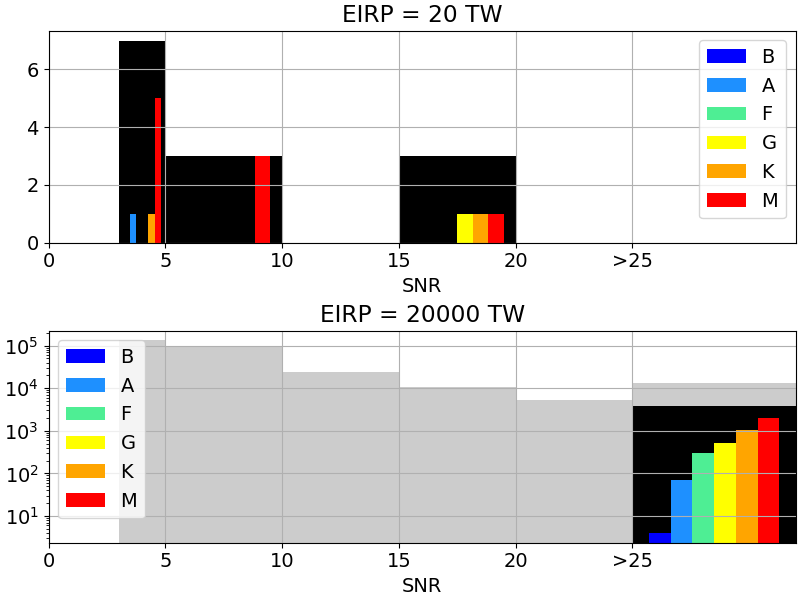
\includegraphics[width=0.75\linewidth]{figures/catcounts.png}
    \caption{Detection counts for the Breakthrough Listen target selection for nearby stars \citep{2017PASP..129e4501I} and a catalog of stars within 100 light years (https://chview.nova.org/solcom) for an ``Arecibo'' scale transmitter (top) and 1000 times larger (bottom).  The black background is the total number per signal-to-noise ratio bin and the colors are the individual spectral types.  The first bin extends from 3-5 and the last bin is 25 and greater.  The light gray on the bottom plot shows the shows the same calculation for all of the stars in the Gaia Nearby Start Catalogue \citep{2021A&A...649A...6G}}
    \label{fig:isaacsonetal}
\end{figure}

% Paragraph below is now redundant.
% Signals of interest must be carefully sought within this cacophony of RFI. To differentiate between RFI and a technosignature requires that the technosignature signal is at a frequency/time not inhabited by RFI and the signal must persist and be quite stable over a timeframe of many minutes.  The signals are assumed to be nearly monochromatic and slow-drifting in time.  A series of on-off measurements are used (for single-dish experiments)to make sure that the signal-of-interest is coming from the main beam of the telescope and not RFI in a distant sidelobe.  These techniques are incredibly powerful in conducting senstive searches over the available bandwidth, and have the added benefit being able to use very large earth-based telescopes to dramatically increase the sensitivity.  However, many limitations exist on appropriate ranges of frequency and time, and some frequency ranges are so impacted that searches (and radioastronomy research generally) are infeasible in those bands.  Signals of short duration (a few seconds) or signals heavily modulated are nearly impossible to discern.  And of course, technosignatures ``behind'' RFI is not detectable (or at least believably so).

\begin{figure}
    \centering
    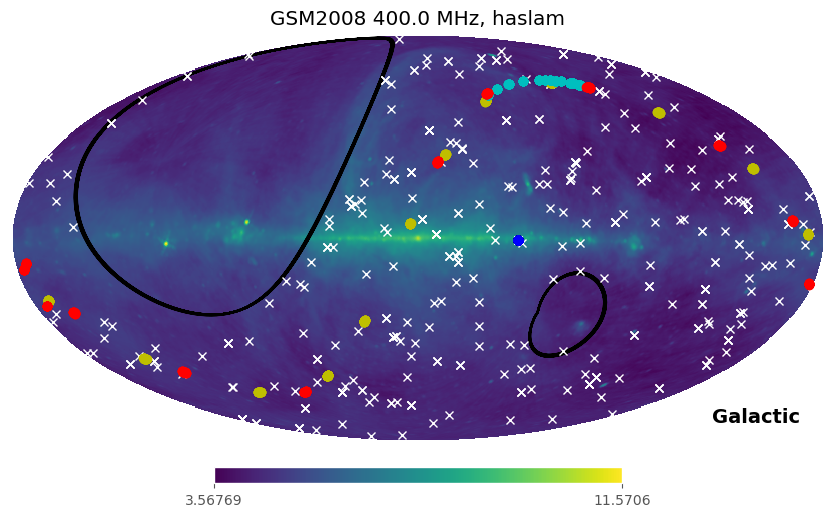
\includegraphics[width=0.95\linewidth]{figures/galaxy_plot.png}
    \caption{Graphic showing the field-of-view of LFT3 over a month imposed over a graphic of the Milky Way at 650 MHz.  The white point's are all of the stars within 10pc within the field-of-view, the blue dot is Alpha Centauri, the yellow dots are the monthly ecliptic points over the year 2028, red dots are Mars over that period and the cyan dots are Jupiter.}
    \label{fig:fieldofview}
\end{figure}

%With online beamforming capabilities we can search the nearest stars  across a range of frequencies rarely searched from Earth but represent some of our most power transmitters \citep{Tremblay_2022}. Within the current FPGA framework, calibration and dynamic spectrum creation can be completed giving us access to the full details of the signals detected for each frequency range. This combined with a sample of the time-averaged spectrum will provide a unique dataset in which to seek an answer to ``Are we alone?". Assuming a civilization is capable of building a big dish to generate an isotropically distributed signal of $\sim$10${^17}$\,W, with a 6$\sigma$ sensivity of 0.5\,Jy, we could expect to detect that signal out to about 3\,pc. However, a beamed signal or a large megastructure is expected to create power over 10$^{26}$\,W. 

%The $Gaia$ Space telescope has given has a large catalog of targets which we are already using in blind, commensal surveys with MeerKAT (Czech et al. in prep) and the Karl G. Jansky Very Large Array \citep{Tremblay_2024}. From this experience we can develop and efficient search working on the FPGA framework.

\textbf{Science Specifications:} As shown in Figure \ref{fig:bubbles}, the proposed telescope frequency covers a new parameter space in technosignature searches, especially with the low- and mid-band receivers. The technosignature science case requires some in-line processing of the data to find signals of interest and generation of dynamic spectra or raw voltage postage stamps around signals of interest. On the commensal, real-time system at MeerKAT and the VLA \citep{Tremblay_2024} we use \textsc{seticore}\footnote{\url{https://github.com/lacker/seticore}} to search for the signals toward beamformed targets. \textsc{seticore} uses an efficient Taylor-Tree dedispersion algorith to autonomously search for narrowband signals. The user specifies the signal-to-noise ratio to identify signals of significance and the drift rate search width. To save on information needing to be transfered to the ground, instead of sending the dyanmic spectrum, we can de-disperse the signal and only transmit the time averaged power spectrum. 

As there is no known signal thus far identified, the frequency resolution and time resolution are open parameters that are flexble to needs to keep data rates and processing to a minimum. However, most of current radio astronomy experiments utilize $<$10\,Hz frequency resolution. 

We can verify these modes of operation by looking toward Mars where there are number of space-based and ground-based communication signals heading back to Earth on a regular basis. The carrier signals are often emitted at around 2~GHz and represent a population of narrow-band artificial signals.

\subsection{Transients}
In the last 20 years the field of radio transients (both slow and fast) has brought a wealth of information, significantly advancing various areas of physics. Notably, pulsars and fast radio bursts (FRBs) stand out due to their unique potential to reveal new kinds of physics \citep{beskin_radio_2015, ng_brief_2023}. These astrophysical phenomena offer valuable insights into gravitational waves, cosmology, and plasma physics, among other fields. However, radio observations can also shed light on other transients such as flare stars and planetary conditions within the solar system. Overall, the strength of a lunar-based telescope is in discovering the unknown. This includes the possible detection of various `low-D' (or dispersion measure, an indicator of relative proximity) events, on timescales of milliseconds to minutes: low-DM FRB analogues, FRBs from Galactic magnetars, decimetric solar bursts, stellar bursts, and undiscovered time-domain phenomena. In particular, the discovery of new populations of transient astrophysical sources in the very local Universe at 0--30~MHz and 87--108~MHz. Figure \ref{fig:transient_space} details various observational setups of LFT3 against well known transients on the $\nu \text{W}$ vs $L_\nu$ parameter space. 

\begin{figure}[!ht]
    \centering
    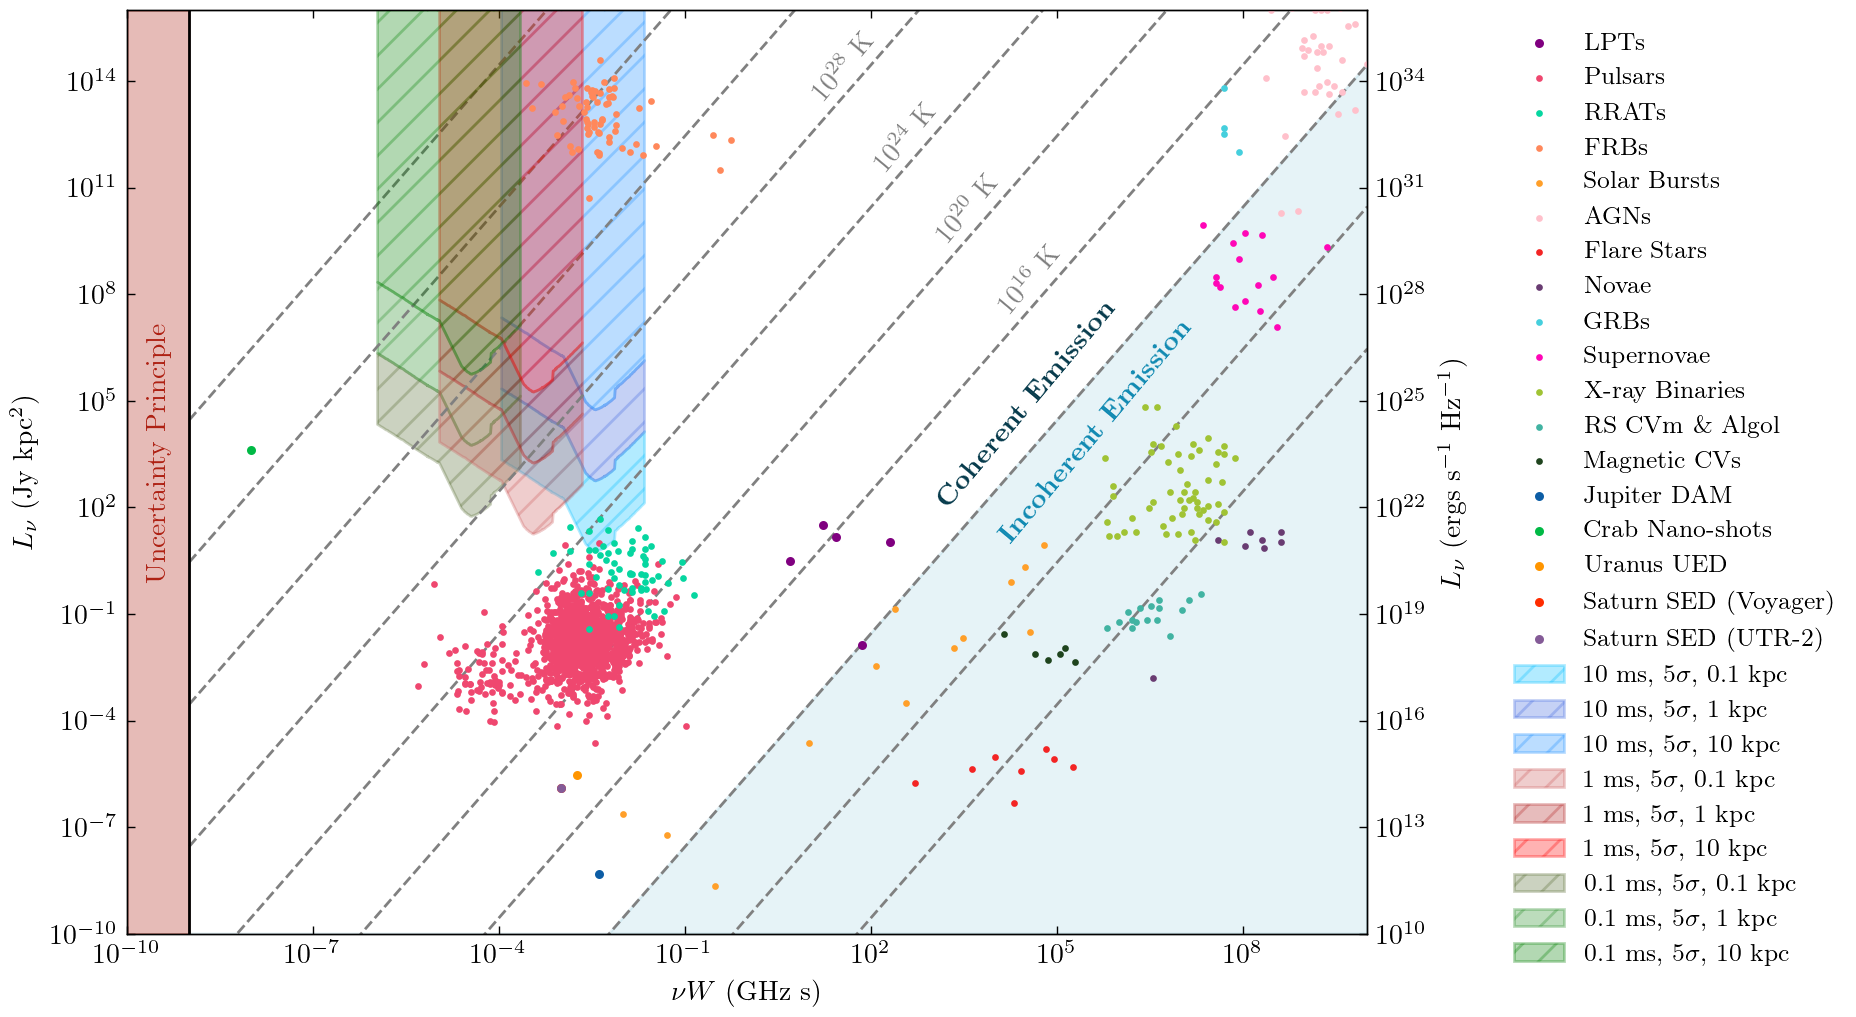
\includegraphics[width=0.8\textwidth]{figures/phase_space.png} 
    \caption{Transient Parameter Space figure adapted from \citet{pietka}. This plot illustrates the sensitivity regions of a LFT3 observational setup across different pulse widths (0.1~ms, 1~ms and 10~ms) at 1~kpc on a $\nu \text{W}$ vs. $L_\nu$ phase diagram. Where $\nu \text{W}$ represents the product of observed frequency and pulse width and $L_\nu$ shows the spectral luminosity. The the blue, green and red hashed regions correspond to a pulse width and show the detectable signal levels above a threshold of $5\sigma$ for the LFT3 bandwidth.}
    \label{fig:transient_space}
\end{figure}





% Emission from planets has also been observed in the form of auroral emission. The most notable example of this is the Jovian system. The Jovian system is known to have auroral emission that is driven by the interaction of the solar wind with the magnetosphere of the planet. Coherent radio emission from the aurora is thought to be produced through the cyclotron maser instability \citep[ECM;][]{zarka_auroral_1998} which injects a high-velocity electron population into the magnetosphere. The maximum frequency of the ECM is directly proportional to the magnetic field strength of the object at its emitting point \citep{kavanagh_hunting_2023, joe_nature_review}.


\subsubsection{Solar Physics}
Low-frequency studies of the Sun date back to the earliest days of radio astronomy, with some of the first published observations appearing in 1963~\citep{Wild_1963}. Despite this early start, a new generation of instruments, including LOFAR and the MWA, has enabled significant advances due to wider bandwidths, improved telescope design, and enhanced computational capabilities. Key science goals include the study of non-thermal emissions, gyrosynchrotron emission associated with coronal mass ejections (CMEs), targeted analyses of solar bursts (Types I--V), and polarimetric measurements. Many of these studies require high-bandwidth imaging on short time scales~\citep{Kansabanik_2022}, though spectral-temporal characteristics of quiescent versus active solar states are also of interest given their impact on Earth-based technologies.

One of the significant outstanding questions in heliophysics is: ``How does the Sun produce strong southward-pointing magnetic fields in solar CMEs that lead to geomagnetic storms? How can solar and geomagnetic super-storms be predicted?'' In an effort to explore the connection between CMEs and phenomena such as Type II bursts, solar flares, and shocks, \citet{Bastian_2001} analyzed observations at 150 and 450\,MHz with 32\,s integration and $\sim$1\,MHz spectral resolution. Their work yielded constraints on thermal plasma density, density filling factors, relativistic electron number density, and magnetic field strength within CMEs—values still widely referenced today.

The electron cyclotron maser instability~\citep[ECMI;][]{EMI}, a plasma instability occurring in magnetized environments with energetic electron populations, is thought to be a key emission mechanism in both solar and stellar contexts. ECMI is considered the primary driver of coherent radio bursts observed during Type II and III solar events, where electron beams accelerated in the corona generate strong, polarized emission. Understanding the conditions that trigger ECMI and the characteristics of the resulting emission is essential for studying solar radio physics at low frequencies.

Solar observations at varying time and frequency resolutions remain challenging. A farside lunar telescope would offer a dynamic spectral view of solar activity across a frequency range unobservable from Earth and not explored in detail since the Voyager missions of the 1970s. As the Sun approaches solar maximum, such a telescope would be uniquely suited for capturing transient low-frequency events, such as Type II/III bursts and solar-driven auroral emissions from planetary bodies. 



Interplanetary scintillation (IPS) observations of from the lunar farside could be used to pinpoint solar wind and heliophysical structures, by measurement of the rapid intensity fluctuations of the compact radio background caused by turbulence in density regularities in the solar wind \citep{fallows_application_2023}. This technique could potentially reveal bulk flow velocities and turbulence levels and detect large-scale heliospheric density structures (e.g., tracking CME-driven shocks) throughout the inner heliosphere. Compared to Earth-based IPS experiments \footnote{e.g., with the MWA and LOFAR operating at $80$–$300~\text{MHz}$, \cite{fallows_separating_2016} and \cite{kaplan_murchison_2015}} that are limited by terrestrial ionospheric distortion. LFT3 could lend its low observing frequency phased array to achieve higher angular resolution \citep{DEX}. 




% \textbf{Scientific Specifications:} High-time-resolution dynamic spectra ($\sim$1--2\,ms) with $\leq$0.5\,MHz spectral resolution would significantly benefit the solar physics community. Coordinated observations with other low-frequency instruments, such as the MWA or LOFAR, would provide coverage over a broader spectral range. Such data products would be valuable during both active and quiescent solar phases. The inclusion of Stokes V dynamic spectra at comparable resolution would offer additional diagnostic capability.

\textbf{Scientific Specifications:} High-time-resolution dynamic spectra with time resolution on the order of 1--2\,ms and spectral resolution of $\leq$0.5\,MHz would be critical for resolving fast-evolving solar radio bursts, particularly Type III and ECMI-driven emission structures. Coherent bursts from solar events can reach flux densities of $\sim$10$^3$--10$^6$~Jy, but occur over narrow frequency bands and short durations, requiring fine temporal and spectral sampling for full characterization. Dynamic spectra in both Stokes I and V would allow for polarimetric studies of coronal magnetic fields and emission mechanisms. Low-frequency IPS studies require long integration baselines (e.g., 10--100\,s) across a wide field of view to track scintillation patterns and infer bulk solar wind properties and density turbulence. \

The frequency range of interest spans $\sim$0.1--30\,MHz, encompassing the decametric and hectometric bands relevant for Type II/III solar bursts and the IPS regime. This range lies entirely below the Earth's ionospheric cutoff, making lunar deployment essential. A phased-array configuration with beam steering would facilitate flexible observation of both targeted and wide-field events. Coordinated observations with MWA, LOFAR, and space-based platforms like SunRISE would enable multi-instrument solar diagnostics across a broader frequency range and heliocentric baselines. These data products would be valuable across both active and quiescent solar phases, contributing to long-term solar monitoring and forecasting of geomagnetic activity.


\subsubsection{Solar System Emission} 
There exist numerous sources of radio emission throughout the solar system. Most notably, Jupiter's strong magnetic field interacts with its moons, particularly Io~\citep{Io}, but also Europa and Ganymede~\citep{Corentin} producing intense MJy-level radio emissions. Jupiter emits over a broad frequency range from 10~kHz to 40~MHz~\citep{zarka_auroral_1998}, with its hectometer-wavelength (1--5~MHz) emission modulated by solar wind activity~\citep{Desch1984}. A lunar-based telescope would enable observations of these low-frequency bands, particularly around solar maximum, offering an opportunity to study solar-wind-driven dynamics in the Jovian system. A lunar telescope is also well-suited to probe low-frequency emissions from the outer solar system planets. During its flyby, \textit{Voyager 2} detected strong $\sim$100~Jy radio emissions from both Neptune and Uranus, indicative of the presence of strong planetary magnetic fields \citep{zarka_auroral_1998, ZHANG199237}. One high-priority science case is the re-detection of low-frequency radio emission from Uranus and Neptune. Voyager's low-band instrument also observed emissions associated with lightning activity (0.1--1~MHz) on Uranus~\citep{1986Zarka_Emission}. Despite subsequent attempts using LOFAR and NenuFAR, this emission has not been detected again likely due to the ionosphere. A confirmed re-detection would carry significant implications for understanding planetary atmospheres, magnetospheres and general nature of the weather on planets in the outer Solar system. Saturn's lightning-induced radio emissions, which span from 2 to 30~MHz and reach intensities of $\sim$1000~Jy, present another valuable target for low-frequency monitoring~\citep{Zarka2004}.

\textbf{Scientific Specifications:} Dynamic spectra in Stokes I and V with high time resolution (e.g., sub-second to a few seconds) would enable characterization of emission morphology and polarization. Known radio flux densities from outer solar system planets span a wide range, from $\sim$X~Jy (Uranus, Neptune) to $\sim$X~Jy (Saturn lightning), and up to MJy levels for Jupiter~\citep{zarka_auroral_1998,ZHANG199237,Zarka2004}. Emission is typically concentrated between 0.1–40~MHz, a range that lies mostly below the Earth's ionospheric cutoff. For Neptune and Uranus, emissions associated with lightning and auroral activity are expected around 0.1–1~MHz with burst durations of seconds to minutes~\citep{1986Zarka_Emission}, requiring longer integration times and high spectral resolution (e.g., $\leq$100~kHz). A bandwidth covering at least 0.1–30~MHz is necessary to capture the full spectral envelope of outer planet emissions. Additionally, dual-polarization capability is critical for distinguishing between thermal and non-thermal processes and identifying strongly polarized bursts.



\subsubsection{Flare Stars}

Radio flare stars, often young, magnetically active stars, provide insight into stellar magnetic activity, star formation, and the early stages of stellar evolution. Observations from a farside lunar telescope could reveal details about the mechanisms driving these flares and their impact on the surrounding stellar environment. Studying radio flare stars also has implications for exoplanetary science. The intense radiation from these flares can affect the habitability of orbiting exoplanets. Flare stars can also be used as a means to study stellar-exoplanet interactions \citep{joe_nature_review}. A farside lunar telescope lends itself to assess the radiation environment of these planets, contributing to our understanding of exoplanet habitability based on the low frequency window observed and the unique RFI environment that the farside has.

Observing these stars, especially at low frequency ($\leq 300$ MHz) act as probes into stellar and planetary plasma environments. Coronal Mass Ejections (CMEs) have a low-frequency burst component in which information about the kinematics of plasma can be deduced \citep{villadsen_ultra-wideband_2019}. Incident solar wind is also the primary driving force of auroral emission on magnetized planets. Radio emission from stars is typically produced through CMEs, observed phenomenologically in the Sun as type II and III solar bursts. They are also very radio loud stars like CR Draconis peaking at 200~mJy at low frequencies \citep{callingham_low-frequency_2021} making their detection a viable science goal of LFT3. 

Much time has been spent observing Ultracool Dwarfs (M7) as they provide a good analogue to the Jovian systems. This allows for direct comparison between the two.  This provides valuable insights into the formation and atmospheric processes. Moreover, such comparative studies contribute significantly to the understanding of planetary evolution and diversity beyond our immediate neighborhood. Recent detection of radiation belts around a UCD further supports the analogy to Jupiter, as radiation belts are a key characteristic of Jupiter's magnetosphere \citep{joe_nature_review}. \ UCDs, being intermediate in mass between stars and planets, serve as a bridge to understanding exoplanet detection. The discovery of bursting radio emission from a brown dwarf and subsequent detections in UCDs indicate departures from established stellar coronal/flaring relationships. \ Radio bursts from UCDs can exhibit periodic timing \citep{hallinan_rotational_2006} along with strong circular polarization and high brightness temperatures, suggesting the involvement of the ECM process in generating radio emission. Despite a significant amount of gigahertz-frequency radio searches, detection rates for UCD radio emissions remain stubbornly low at around 10\% overall at higher frequencies \citep{lynch_radio_2016}. Given that LFT3 will observe unique and low frequencies there significant insights observing at frequencies sub 300 MHz can uniquely constrain the magnetic field strengths near the emission region of UCDs, offering insight into field geometry and strength not accessible at higher GHz frequencies. 



\textbf{Scientific Specifications:} As mentioned flare stars a radio loud on the scale of 10's of mJy's at lower frequencies \citep{driessen_sydney_2024}. This puts nearby flare stares well within the realms of detection. As with the other science cases LFT3 allows for observations in previously contaminated or unreachable frequencies, specifically FM and sub 30~MHz band will be on interest for monitoring already known bright sources \citep{joe_nature_review}. Time resolution of $\leq$100\,ms and spectral resolution of $\sim$0.1--0.5\,MHz would enable detection and classification of coherent bursts, including ECMI-driven emission. Dual-polarization capability will be important to detect and analyze strongly circularly polarized bursts, which are diagnostic of magnetic field geometry and strength in stellar objects. 


\subsubsection{Pulsars}
Pulsars are highly magnetized, rotating neutron stars that emit beams of electromagnetic radiation from their poles analogous to a lighthouse. These cosmic lighthouses serve as precise cosmic clocks, providing insights into the interstellar medium, gravitational waves, and the fundamental physics of matter under extreme conditions \citep{pulsar_handbook, agazie_nanograv_2023}. It is theorized that pulsars start off spinning rapidly when they are created, but their rotation slows over time due to the combined effects of electromagnetic radiation, the pulsar wind, and possibly gravitational waves, as well as changes in the surrounding medium, which can also alter the structure of the pulses \citep{LW_2013}. By using coherent dynamic spectra, sensitivity to weak pulses can be improved, and frequency and time resolution can be adjusted to decrease the effects of dispersion measure smearing (e.g. \cite{WL_2020}). Figure \ref{fig:transient_space} shows the average values for a pulsar population luminosity distribution, but single pulses can extend several orders of magnitude higher \citep{karuppusamy_giant_2010}. LFT3 won't see every pulse from a pulsar, but single pulse observations will yield a wealth of information (i.e. period, profile, phase, width, etc.). 


Broadband studies of pulsars allow for a study of the emission physics and surrounding material, where the lower frequencies are sensitive to emission closer to the pulsar surface \citep{hassall_wide-band_2012}. With ground-based radio telescopes, the ionosphere can create challenges, especially in weaker pulsars that have a peak spectral turn-over between 100--200~MHz \citep{Stappers_2011}. By moving the radio telescope off the Earth, away from the ionosphere cut-off typically around 30~MHz, a broader range of pulsar emission physics can be studied than has not yet been explored. One of the lowest pulsar detections was observed with the Low Frequency Array detecting emission down to 15~MHz with favorable ionospheric conditions \citep{Kondratiev_2012}.

%LFT3 could be well placed to observe some of the brightest pulsars below 15~MHz. 

A farside lunar telescope, shielded from Earth’s radio frequency RFI, would significantly enhance pulsar observations by providing a pristine observational environment. This location allows for low-frequency studies, critical for understanding the early stages of pulsar emission mechanisms and the surrounding interstellar medium. Furthermore, the lunar farside offers an opportunity to continuously monitor pulsars without the interruptions caused by the Earth’s rotation, increasing the data quality and allowing for the detection of subtle changes in pulsar behavior over time \citep{jankowski_spectral_2018}.


\textbf{Science Specifications:} Beamformed data products are highly valuable for discovering a wide range of transient events, with pulsars being one of the potential beneficiaries.LFT3 will provide extensive sky coverage, especially at lower frequencies; however, this comes with a reduced effective area (\(A_{\text{eff}}\)) due to the increased sky temperature (\(T_{\text{sky}}\)) and system noise, which lower the overall sensitivity. Consequently, the pulsar candidates identified by LFT3 will be giant pulses observed at unique frequencies (cite Crab giant pulses). However, the ability to observe pulsar emissions in a pristine environment across a large bandwidth holds significant scientific value on its own. 
%LFT3 can be compared to instruments like Galactic Radio Explorer \citep[GREX;][]{GREX} which is designed to detect FRBs and Magnetar Bursts. 



\subsubsection{Fast Radio Bursts}
Fast Radio Bursts (FRBs) are intense\footnote{Most FRBs have a peak flux of 0.1 Jy to a few 100's of Jy. The brightest ever seen was a Galactic FRB which exhbited MJy emission.}, millisecond-duration radio pulses originating from extragalactic sources. Their origins remain one of the most intriguing mysteries in modern astrophysics. Although Galactic magnetars have shown to exhibit similar FRB-like emission \citep{BC_2020,chime2020sgr1935}, the exact progenitors and emission mechanisms are still unknown. Some bursts are observed from stellar environments which show evidence for recent star formation activity, e.g.~\citet{piro2021}. The stellar environments of other sources such as FRB 20200120E suggest that FRB progenitors may emit bursts long after star formation activity~\citep{kirsten2022m81} has ended, providing evidence for multiple formation channels.

The Canadian Hydrogen Intensity Mapping Experiment (CHIME) telescope is currently the world leader for detecting new Fast Radio Bursts with its 200\,deg$^{2}$ field-of-view and observing frequency of 400--800\,MHz, and outrigger stations for burst localization~\citep{leung2021synoptic,lanman2024kko}. 

Where a low-frequency Lunar telescope can provide a large benefit, is in understanding the true nature and populations of FRBs is through the study of emission at lower radio frequencies with high time resolution, as this is becoming a clear factor in understanding the source populations.LFT3, supplemented by wide field-of-view ground stations on Earth could be used to co-observe to enable micro-arcsecond localisation of the brightest FRBs, something which would be of unprecedented scientific value (see e.g. \cite{nimmo_burst_2023}). 

Currently, the Commensal Real-time ASKAP Fast Transients Collaboration (CRAFT; 700--1.8\,GHz) offer the largest number of localized repeater sources \citep{shannon2024ics, SD_2023}, with some more recent contributions from the Five-hundred-meter Aperture Spherical Telescope (FAST) collaboration \citep[1.00--1.45\,GHz;][]{ZX_2023} and the DSA-110 \citep{LC_2023,sharma2024preferential}. Observing away from RFI, the ionosphere and availing of the FM band may provide key understanding to unlock the true nature and originating source of emission.

Low-frequency observations of FRBs are crucial for understanding their propagation through the intergalactic medium, potentially unveiling the distribution of baryonic matter and offering clues about the emission mechanism and source plasma environments. LOFAR observations of FRB 20180916 have revealed potential evidence for interaction between a neutron star and its binary companion by observing bursts down to 100 MHz~\citep{pleunis2021lofar}.

\textbf{Scientific Specifications:} Detection of FRBs at low frequencies requires high time resolution ($\leq$1\,ms) and sufficient spectral resolution ($\sim$0.1--0.5\,MHz) to resolve dispersion sweeps and intrinsic burst structures. While most FRBs peak between 400--800\,MHz, several have been observed down to $\sim$100\,MHz, with flux densities ranging from $\sim$0.1 to hundreds of Jy~\citep{pleunis2021lofar}. Dual-polarization capability and dynamic spectra in Stokes I and V will support burst characterization. Observations in the sub-100\,MHz range, inaccessible from Earth, may uncover a suppressed or scattered FRB population and place limits on free-free absorption and propagation effects. LFT3's large field of view and ability to co-observe with ground-based arrays would also enhance the chance of real-time detection and sub-arcsecond localization.

% \textbf{CL: It is possible to estimate the FRB rate from CHIME, which detects about 1000 bursts per full year of observation in the same frequency range over a 200 deg$^2$ FoV with a coherent SEFD of 50 Jy. Assuming a Euclidean population of sources, in the coherent FoV of LFT3 of $\sim 4000$ deg$^2$ at the bottom of the mid-band, $\sim 0.88-2.5$ bursts could be detected per year of observation.}



\subsubsection{Long Period Transients}

Galactic long-period radio transients represent a burgeoning new sub-class of transients. Distinguished by their exceptionally long periods, minuter long pulse duration and their low frequency emission. The prototypical example is GLEAM-X J162759.5-523504.3 \citep{hurley_walker_radio_2022}. This object exhibits a period of 18.18 minutes and a pulse duration of $\sim 1$ minute at 100--200~MHz. The measured DM for this source was $\sim57~\text{pc cm}^{-3}$ indicating a Galactic origin. The distribution of pulses seen from this source are orders of magnitude larger (30--60~s) than that of FRBs and have fluxes of 5--40~Jy. This makes them one of the most feasible science goals of LFT3 (see. Fig. \ref{fig:transient_space}). The emission is also highly linearly polarized (90\%) with a spectral index of $\sim 1.2$, suggesting a strongly magnetized engine (reference). It is intially thought that magnetars may be a plausible source for these transients. However, the absence of multi-wavelength emission from these sources contradict many models (references), leaving the discussion for the origin of these transients still on the table. Subsequent surveys have revealed more of these objects with periods ranging from minutes to hours(reference). Notably they show low dispersion measures ($\lesssim$ few $10^2~\text{pc cm}^{-3}$) which make them relatively easy to distinguish from when observing at low frequencies. They sources are not exceedingly rare and harbor many open questions yet to be fully explored. \\ 
LFT3 presents a unique opportunity to advance this field while it's still in its infancy. As previously discussed having broadband observations of these sources in an RFI pristine environment will give further insight to these objects. Such observations could reveal whether these ultra-long-period objects exhibit even longer-wavelength emission, test how their spectra evolve, and potentially catch new transients with ultra-low dispersion measures in the local Galaxy.

\textbf{Scientific Specifications:} Long-period transients, with pulse durations of 30--60\,s and peak flux densities ranging from 5--40\,Jy at 100--200\,MHz~\citep{hurley_walker_radio_2022}, are well within the detection capabilities of LFT3. Observations should include dual-polarization data to capture the high linear polarization fraction ($\sim$90\%), with spectral resolution of 0.1--0.5\,MHz and time resolution on the order of 1--5\,s to resolve burst profiles while preserving sensitivity to slow periodicity. The observed low dispersion measures ($\lesssim$200\,pc\,cm$^{-3}$) reduce computational demands for de-dispersion, enabling efficient real-time searches. 

\begin{deluxetable*}{ccccccc}
    \tablecaption{Minimum Detectable Flux Densities ($S_{\text{min}}$) Grouped by pulse width.\label{tab:smin} for 48 element Vivaldi phased array feed.}
    \tablehead{
    \colhead{Pulse Width} &
    \colhead{Frequency} &
    \colhead{Wavelength} &
    \colhead{$A_{\text{eff}}$} &
    \colhead{Gain} &
    \colhead{SEFD} &
    \colhead{$S_{\text{min}}$} \\
    \colhead{(ms)} &
    \colhead{(MHz)} &
    \colhead{(m)} &
    \colhead{(m$^2$)} &
    \colhead{($10^{-4}$\,K/Jy)} &
    \colhead{(kJy)} &
    \colhead{(Jy)}
    }
    \startdata
    \textbf{0.1}   & 250 & 1.2 & 17.1 & 6.2 & 16.2  & 572.5 \\
                   & 500 & 0.6 & 4.3  & 1.5 & 64.8  & 2290.2 \\
                   & 750 & 0.4 & 1.9  & 0.7 & 145.7 & 5152.9 \\
    \hline
    \textbf{1}     & 250 & 1.2 & 17.1 & 6.2 & 16.2  & 181.1 \\
                   & 500 & 0.6 & 4.3  & 1.5 & 64.8  & 724.2 \\
                   & 750 & 0.4 & 1.9  & 0.7 & 145.7 & 1629.5 \\
    \hline
    \textbf{10}    & 250 & 1.2 & 17.1 & 6.2 & 16.2  & 57.3 \\
                   & 500 & 0.6 & 4.3  & 1.5 & 64.8  & 229.0 \\
                   & 750 & 0.4 & 1.9  & 0.7 & 145.7 & 515.3 \\
    \hline
    \textbf{100}   & 250 & 1.2 & 17.1 & 6.2 & 16.2  & 18.1 \\
                   & 500 & 0.6 & 4.3  & 1.5 & 64.8  & 72.4 \\
                   & 750 & 0.4 & 1.9  & 0.7 & 145.7 & 162.9 \\
    \hline
    \textbf{1000}  & 250 & 1.2 & 17.1 & 6.2 & 16.2  & 5.7 \\
                   & 500 & 0.6 & 4.3  & 1.5 & 64.8  & 22.9 \\
                   & 750 & 0.4 & 1.9  & 0.7 & 145.7 & 51.5 \\
    \hline
    \textbf{10000} & 250 & 1.2 & 17.1 & 6.2 & 16.2  & 1.8 \\
                   & 500 & 0.6 & 4.3  & 1.5 & 64.8  & 7.2 \\
                   & 750 & 0.4 & 1.9  & 0.7 & 145.7 & 16.3 \\
    \enddata
    \tablecomments{
    Minimum detectable flux densities are calculated assuming a system temperature of 100\,K, a bandwidth of 100\,MHz, and a signal-to-noise ratio of 5$\sigma$.
    }
\end{deluxetable*}
    
    
    
    

\subsection{Spectral Lines}
Radio frequency interference has significant impact when studying Galactic and extragalactic chemistry, especially in the frequency range around 1\,GHz (e.g. \citealt{Liang_2023}). This is due to an increasingly cluttered frequency band of intense signals from anthropengenic RFI, often leaking into protected radio astronomy bands. This impacts our ability to study the chemistry, kinematics, and age of astronomical objects through the spectral properties of atoms and molecules. Therefore, we must look to more creative ways of studying the Galaxy to study the dynamical motions and slow changes that are happening over the life-spans of stars and galaxies, a crtical aspect for understanding their evolution.

\subsubsection{Extra-galactic HI}
Hydrogen is one of the most prominent elements in the Universe and the neutral hydrogen line at 21\,cm (1.420\,GHz) is one of the most prominent diagnostic lines used in radio astronomy. From testing models of the early Universe to tracing the spiral arms of our Galaxy, H{\sc I} is an important line for understanding motions and dynamics. However, on Earth, even though the spectral region around the 1.42\,GHz emission is protected and reserved for radio astronomy, the spectral region around the line is heavily polluted with RFI. This makes studying galaxies within our local Universe and beyond challenging. 

The neutral hydrogen line at 1.42\,GHz shifts to lower frequencies as a function of distance from the study of our own Galaxy to the epoch of reonization (the birth of the first stars) proposed to be around 150\,MHz. Although the studies of the earliest time-lines of our Universe employ a unique set of techniques to look for the neutral hydrogen spectral signature, the techniques used to study out to around a red-shift of two employ standard spectral emission detection techniques (i.e. \citealt{WALLABY,FLASH}). This means looking for an absorption or emission line, often a few 100kHz wide, in the spectral data after time-averaging. We use the H{\sc I} signature to study the age, dynamics, mass of galaxies, a measure of dark matter, and much more. Therefore, moving the telescope away from the Earth-based interference has immediate benefit of being able to study objects without the concern of RFI imapacting the calculations and intrepeations of the objects properties.

\textbf{Scientific Specifications:} For this work, the data product would need to be a time-averaged power spectrum of beamformed targets or incoherent sum. The spectral resolution of a 100kHz would be sufficient due to the rapid rate of rotation in nearby galaxies with no specification on time assuming the source is still within the FOV. However, if the focus is on more distant galaxies and then a 1kHz frequency resolution would be preferred. 

\subsubsection{Radio Recombination Lines}
The diffuse cold neutral medium (CNM; T$_{s}$ $<$ 100\,K) is an important component of the interstellar medium (ISM). To date this gas has been primarily studied using the HI 21 cm line in absorption \citep{Dickey_1990}. The low ionization potential of carbon (11.4\,eV) permits carbon atoms, in the form of cold radio recombination lines (CRRL), to be ionized by the far-UV radiation fields. A second powerful and complementary probe of the conditions in the neutral ISM is provided by the CRRLs that arise in this ionized gas. CRRLs at low radio frequencies ($<$ 1.5 GHz) have been detected in the Galactic plane in both emission and absorption with a number of telescopes (e.g. \citealt{Kantharia_2001,Salas_2019,GDIGS}). 

At large n-bound states, observed at frequencies less than 100 MHz, the relative populations of atomic levels are controlled primarily by collisional processes \citep{Tremblay_2018}. This makes it the population levels close to the kinetic temperatures of less than 100\,K and so the lines are detected in absorption along the line of sight towards strong continuum sources. The population becomes inverted at lower n-bound states at frequencies greater than 200/,MHz, resulting in emission lines being detected \citep{Gordon-RRL}. In the range of 100 to 200\,MHz, the conversion will take place at a frequency and intensity dependent upon the temperature and density of the gas within the cloud. This means that the more dense the gas, the conversion will shift toward higher frequencies. This makes CRRLs excellent pressure and temperature probes of the ionized gas regions of the ISM \citep{Salas_2019}.

The ionosphere negatively impacts scientific measurements as a wavelength squared dependence, thus having a greater impact on lower frequency observations. Observing low-frequency ($<$500\,MHz) CRRLs is critical in understanding the temperatures and conditions of the ionized gas fronts in the cold gas \citep{Salas_2018}. By removing the telescope from the ionosphere, potential artifacts and features in the spectral data that are not real would be removed, as well as the possibility of artificial spectral broadening, which could change the measured conditions.

\textbf{Scientific Specifications:} The CRRLs will change in width depending on the frequency of detection and the conditions of the environment. However, a 0.5\,kHz resolution would be sufficient to study the lines across proposed frequency bands. Additionally, the data need to only have a 8--10\,second time resolution but more time can be averaged together to increase senitivity, for as long as the sources is in the FOV. We do this with non-moving dipoles with ground-based telescopes by either employing fringe tracking or by doing short time-recordings, correcting for the source position, and then time-averaging the data. If treating the dipoles as independant entities, correlated visbilities would allow for a low resolution map of the regions where the signals are detected. However, beamforming can be used if either the location of the source is known or in an incoherent beam where the lines are particularly strong. Overall, spatial resolution of one degree on the sky would allow for follow-up by ground-based telescopes where more detail is required. The preferred output is a time-averaged power spectrum or a spectrum converted to intensity in Jy. Either way, a calibration of the flux density values will be needed.

\subsubsection{Cosmology}
Except for one singular event that occurred 380,000 years after the Big Bang (the recombination of the intergalactic medium into hydrogen resulting in the cosmic microwave background surface of last scattering, or CMB), red-shifted hydrogen is the only way to learn about large-scale cosmic structure for the next roughly 13 billion years of cosmic evolution (see e.g. \citealt{Fialkov_2024}).  Of particular interest is the rise of astrophysical structure in the cosmic fabric beginning about 13 billion years ago.  Since this signal emanates from a distance of 13 giga-lightyears (Gly), it is exceedingly faint, requiring extreme sensitivity and radio-quiet conditions.  Since the signal of interest is also global, a single antenna is technically sufficient.  Figure \ref{fig:cosmo_h}) shows a cartoon of cosmic evolution as a function of cosmic age and redshift, and maps that to the observed frequency of redshifted hydrogen (yellow line).

The sky is extremely bright, ranging from about 100K to $10^6$k depending on frequency and location, while the signal of interest is milliKelvin, hence the difficulty in making the measurement.  Figure \ref{fig:global_T_bw} shows one model (taken from \citealt{Fialkov_2024}) across frequency (and hence cosmic time).  Note that the observable is the difference between the hydrogen spin temperature and the CMB temperature and may be positive or negative.

\begin{figure}[h]
    \centering
    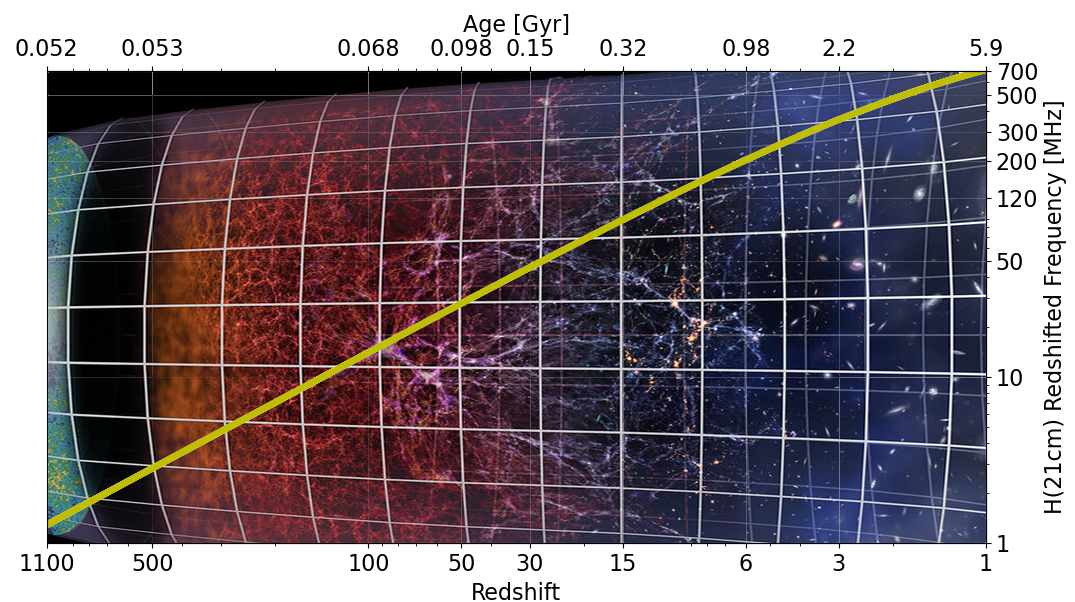
\includegraphics[width=0.8\textwidth]{figures/zage_lft3_python.png}
    \caption{Cosmic evolution and observability by red-shifted hydrogen.  The underlying cartoon (credit: ESO/M. Kornmesser) shows a depiction of cosmic evolution from the era of the cosmic microwave background to the near-monder era.  The top horizontal scale shows time after the Big Bang in Gyr and the bottom the associated red-shift.  The yellow line and vertical axis indicate the observable frequency at that age.}
    \label{fig:cosmo_h}
\end{figure}

\textbf{Scientific Specifications:} 
The expected signal is thermal however that thermal profile changes with cosmic time and hence frequency, so the bandwidth and binning impact the result (see e.g. \citealt{2017PASP..129d5001D}).  Figure \ref{fig:global_T_bw} shows the impact of using 1 MHz and 10 MHz bands for this model and indicates that a bandwidth of a few MHz is desired\footnote{Using as large of a bandwidth as possible is desired, since that reduces the thermal noise.}.
Given the noise of the Galactic plane and the Sun, it is preferable to observe when both are below the horizon.

\begin{figure}[h]
    \centering
    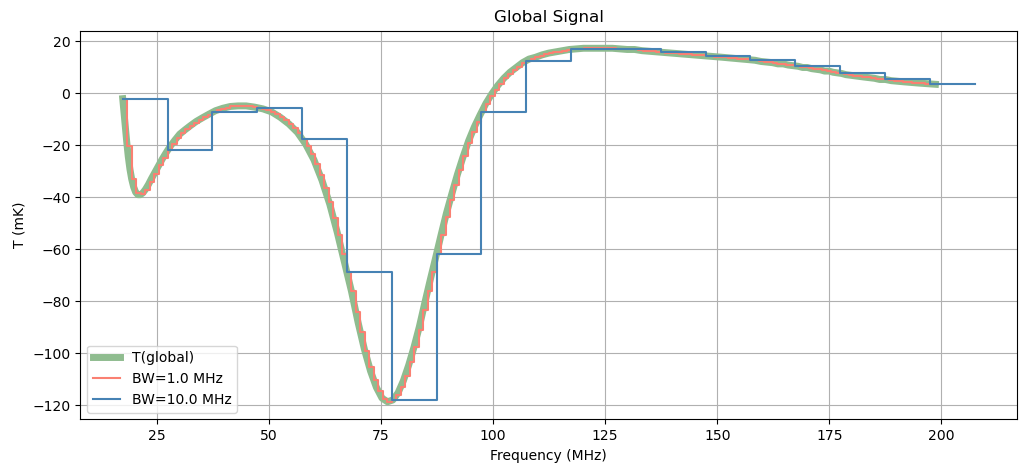
\includegraphics[width=0.8\textwidth]{figures/global_with_bw.png}
    \caption{Global signal from the early Universe.}
    \label{fig:global_T_bw}
\end{figure}

\subsection{Lunar Environmental Observation}

\subsubsection{Spectral Monitoring}
Although the lunar farside should be a pristine RF environment, there will be the potential of some RFI from the communication orbiters that will be in place, as well as spacecraft that are at distances further than the moon.  There is also the potential of unknown actors emitting radio frequencies.  During the LFT3 operational period there is also the potential of additional payloads being deployed, for example China's orbiting interferometer called Discovering the Sky at the Longest Wavelengths (DSL).  Measuring a legacy spectral baseline as well as the potential increasing emergence of RFI is a key objective.

% \begin{figure}[h]
%     \centering
%     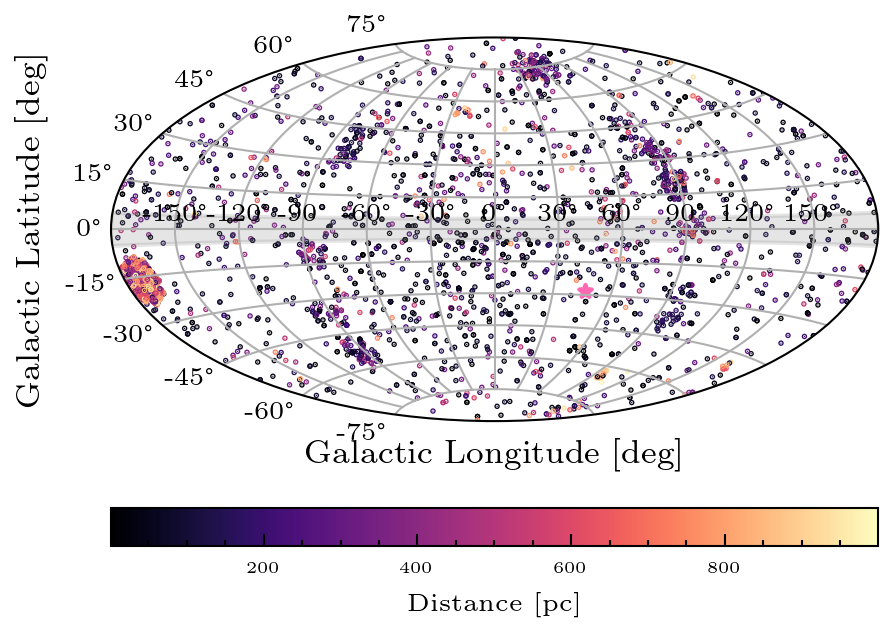
\includegraphics[width=0.6\textwidth]{figures/galactic_projection_NEA.png}
%     \caption{Some plot here with target of intrests that fall within the zenith pointings and their associated Jy measurements based on Tsys etc. }
%     \label{fig:enter-label}
% \end{figure}

\subsection{Operation's Research}
By operating a telescope on the moon, there is a wealth of information that can be gathered scientifically and about the engineering. Through this we can answer questions such as:

\begin{itemize}
    \item The lunar surface topography, conductivity, radiation, and bounce back of radiation and its impact on the scientific results.
    \item We can learn how to do astronomy from the moon and its challenges scientifically. 
    \item How long could the equipment last in the environment? What is the limiting factor for this?
\end{itemize}

\subsection{Science Summary}
%--What is the simplest system we could do science with.  etc.\\
%--Science verification
\subsubsection{Minimum System for Science}
The strength of a lunar farside telescope lies in its ability to uncover the unknown. It is certain that discoveries will be made regardless of the final system design, away from the influence of RFI and the ionosphere. However, depending on the final system design a number of science goals can be completed, as outlined in the sections above. The following are some highlights of science that could be completed with a simpler system. 

One example is only having access to an incoherent sum. This is similar to a single-dish telescope where there is no ability to pinpoint the exact location outside the field of view of the telescope itself. The time and frequency dynamic spectrum, combined with a catalog of the sources within the field, will still provide some indication of the type of event we are seeking to study. 

Provided we continue with a multibeam array as indicated in Figure \ref{fig:midband_beam_maps}, then a range of frequency and time resolutions will provide interesting results. Experiments such as technosignature searches can take on a range of different characteristics and can be easily molded to fit the system limitations. On the other hand, searches for FRBs may require a rigid approach to detect them and their analogs. When studying the solar system, we have little experience studying our planetary neighbors at the lowest radio frequencies, but studying lightning storms and other dynamic phenomena can benefit from the highest time resolution.  

Overall, no matter what the final system design allows, wonderful new discoveries will be made.


\begin{table}
\centering
\caption{A table summarizing the requirements for each science case.}
\begin{tabular}{|l|llll|l|} 
\hline
\textbf{Science Case} & \textbf{Receiver Band} & \textbf{Freq. Res.} & \textbf{Time Res.} & \textbf{Targets}                                           & \textbf{Note}                                                                                         \\ 
\hline
Technosignature       & Low                    & 10Hz                & 0.2-0.5sec         & Gaia Stars                                                 & \multirow{3}{*}{\begin{tabular}[c]{@{}l@{}}Flexible on time and \\frequency resolution\end{tabular}}  \\
                      & Mid                    & 10Hz                & 0.2-0.5sec         & Gaia Stars                                                 &                                                                                                       \\
                      & High                   & 10Hz                & 0.2-0.5sec         & Gaia Stars                                                 &                                                                                                       \\ 
\hline
Pulsar                & Low                    & 0.5MHz              & 1ms                & Blind Search                                               & \multirow{3}{*}{Can target known pulsars}                                                             \\
                      & Mid                    & 0.5MHz              & 1ms                & Blind Search                                               &                                                                                                       \\
                      & High                   & 0.5MHz              & 1ms                & Blind Search                                               &                                                                                                       \\ 
\hline
FRB Analogs           & Low                    & 0.5MHz              & 10ms               & Blind Search                                               & \multirow{3}{*}{\begin{tabular}[c]{@{}l@{}}Need some small DM \\search in realtime\end{tabular}}      \\
                      & Mid                    & 0.5MHz              & 10ms               & Blind Search                                               &                                                                                                       \\
                      & High                   & 0.5MHz              & 10ms               & Blind Search                                               &                                                                                                       \\ 
\hline
Flare Stars           & Low                    & 0.5MHz              & 1sec               & Gaia Stars                                                 & \multirow{3}{*}{\begin{tabular}[c]{@{}l@{}}Addition of Stokes V \\enhances science\end{tabular}}      \\
                      & Mid                    & 0.5MHz              & 1sec               & Gaia Stars                                                 &                                                                                                       \\
                      & High                   & N/A                 & N/A                & N/A                                                        &                                                                                                       \\ 
\hline
Solar System          & Low                    &                     &                    & Local Planets                                              & \multirow{3}{*}{\begin{tabular}[c]{@{}l@{}}Addition of Stokes V \\enhances science\end{tabular}}      \\
                      & Mid                    &                     &                    & Local Planets                                              &                                                                                                       \\
                      & High                   & N/A                 & N/A                & N/A                                                        &                                                                                                       \\ 
\hline
Studies of the Sun    & Low                    & 0.5MHz              & 1--2ms             & Sun                                                        & \multirow{3}{*}{\begin{tabular}[c]{@{}l@{}}Addition of Stokes V \\enhances science\end{tabular}}      \\
                      & Mid                    & 0.5MHz              & 1--2ms             & Sun                                                        &                                                                                                       \\
                      & High                   & N/A                 & N/A                & N/A                                                        &                                                                                                       \\ 
\hline
HI Studies            & Low                    & N/A                 & N/A                & N/A                                                        &                                                                                                       \\
                      & Mid                    & 1kHz                & 5--8sec            & Radio Galaxies                                             &                                                                                                       \\
                      & High                   & 1kHz                & 5--8sec            & Radio Galaxies                                             &                                                                                                       \\ 
\hline
RRL                   & Low                    & N/A                 & N/A                & N/A              &                                                                                                 \\
                      & Mid                    & 0.5kHz              & 5--8sec            & SNR\& HMS$^{1}$ &                                                                                                       \\
                      & High                   & 0.5kHz              & 5--8sec            &                                                            SNR\& HMS$^{1}$&                                                                                                       \\
\hline
Cosmology             & Low                    & 1 MHz              & hours                &  Non-Galactic Plane/Sun  &                                                                                                       \\
                      & Mid                    & N/A              & N/A           & N/A &                                                                                                       \\
                      & High                   & N/A              & N/A            &         N/A &                                                                            \\
\hline
\end{tabular}
$^{1}$HMS=High Mass Star formation regions
\end{table}


\subsubsection{Science Verification}

Whenever a new instrument or telescope is brought online, a verification that the sytem is doing what you expect is necessary. Observational radio astronomy has been going on since World War II, creating a vast catalogue of sources and their behaviour. Therefore, we can use a combination of our knowledge of such sources and simultaneous observations with other telescopes to verify the system. 

%PLOTS That could be useful 
% Frequency/Wavelength against Flux Density of Transients -> parameter space plot 
% Variation of Tsys (basically mapping galactic forground) as a function of Lunar Latitude 
% Senstivity as function of integration time 
% Galactic latitude on the x axis, sensitivity on the y, carious longitudes overlapped. 
% Galactic projection plot for areas/exoplanets of intrest, i.e. benchmarking well known targets. 
% Also worth running some numbers to see how much time A team targets are in primary 